% !TeX spellcheck = en_US
\documentclass{article}

\usepackage{graphicx}

\usepackage[cp1250]{inputenc}
\usepackage[lastpage,user]{zref}
\usepackage[table,xcdraw]{xcolor}
\usepackage{pdfpages}
\usepackage{graphicx}
\usepackage[export]{adjustbox}
\usepackage{tabu}

\begin{document}

\vspace*{3ex}
\begin{flushright}
{\large 28 March 2015}
\end{flushright}

\begin{flushleft}
{\large Lukasz W�jcik\\

}
\end{flushleft}

\hskip3cm

\begin{center}

\Large {\bf
	Individual project
}

\Large {\bf
	Cellular automaton
}

\Large {\bf 
	Technical project
}

\vskip2ex

\vspace{50pt}

\includegraphics[width=100mm]{images/mini.png} \\

\end{center}

\vskip20ex
\label{LastPage}
\begin{flushleft}
{\fontsize{10cm}{1em} {\bf Informations}\\
}
\end{flushleft}

\vskip2ex
\begin{flushleft}
{\huge Scheldue\\
}
\end{flushleft}
\begin{center}
\begin{table}[h]
\begin{tabular}{|l|l|}
\hline
\rowcolor[HTML]{BF6969} 
{\color[HTML]{000000} Date} & {\color[HTML]{000000} Stage} \\ \hline
2015-03-12                  & requirement specification    \\ \hline
2015-04-02                  & technical project            \\ \hline
2015-04-23                  & code of modules              \\ \hline
2015-04-30                  & version 0.98                 \\ \hline
2015-05-07                  & version 0.99                 \\ \hline
2015-05-14                  & version 1.0                  \\ \hline
2015-05-21                  & test report                  \\ \hline
2015-06-11                  & acceptation                  \\ \hline
\end{tabular}
\end{table}
\end{center}

\begin{flushleft}
{\huge Document metric\\
}
\end{flushleft}

\begin{table}[h]
\begin{tabular}{|
>{\columncolor[HTML]{BF6969}}l |l|l|l|l|l|}
\hline
\multicolumn{6}{|l|}{\cellcolor[HTML]{BF6969}\textbf{Document metric}}                                                                                                               \\ \hline
\textbf{Project:}       & \multicolumn{2}{l|}{Cellular automaton}          & \cellcolor[HTML]{BF6969}\textbf{Company:} & \multicolumn{2}{l|}{WUT}                                    \\ \hline
\textbf{Name:}          & \multicolumn{5}{l|}{Cellular Automata technical documentation}                                                                                           \\ \hline
\textbf{Topics:}        & \multicolumn{5}{l|}{Technical aspect of project}                                                                                                 \\ \hline
\textbf{Author:}        & \multicolumn{5}{l|}{Lukasz W�jcik}                                                                                                                         \\ \hline
\textbf{File:}          & \multicolumn{5}{l|}{cellular\_automata\_technical\_documentation}                                                                                        \\ \hline
\textbf{Version no:}    & 0.21 & \cellcolor[HTML]{BF6969}\textbf{Status:} & Designing                                 & \cellcolor[HTML]{BF6969}\textbf{Opening date:} & 2015-03-26 \\ \hline
\textbf{Summary:}       & \multicolumn{5}{l|}{Providing technical documentation.}\\ \hline
\textbf{Authorized by:} & \multicolumn{2}{l|}{Wladyslaw Homenda}           & \multicolumn{2}{l|}{\cellcolor[HTML]{BF6969}\textbf{Last modification date:}}              & 2015-04-01 \\ \hline
\end{tabular}
\end{table}
\begin{flushleft}
{\huge Changes\\
}
\end{flushleft}
\begin{table}[h]
\begin{tabular}{|l|l|l|l|}
\hline
\rowcolor[HTML]{BF6969} 
\multicolumn{4}{|l|}{\cellcolor[HTML]{BF6969}\textbf{History of changes}}     \\ \hline
\rowcolor[HTML]{E3DBDB} 
Version & Date       & Who           & Description                            \\ \hline
0.1     & 2015-03-26 & Lukasz W�jcik & Creation of technical documentation sections. Initial planning \\ \hline
0.2     & 2015-03-27 & Lukasz W�jcik & Creation of technical documentation.\\ \hline
0.21     & 2015-03-27 & Lukasz W�jcik & Correction of spelling mistakes. \\ \hline
\end{tabular}
\end{table}
\newpage
\tableofcontents
\vskip5ex
\begin{flushleft}
{\huge Short summary of documentation\\
}
\end{flushleft}
\Large\hspace{15pt}This document is a technical documentation of Cellular automation program.
\newpage

\section{Production model} \par
\Large\hspace{15pt}
Methodology used for implementation is a "Waterfall Model"
\begin{figure}[h!]
		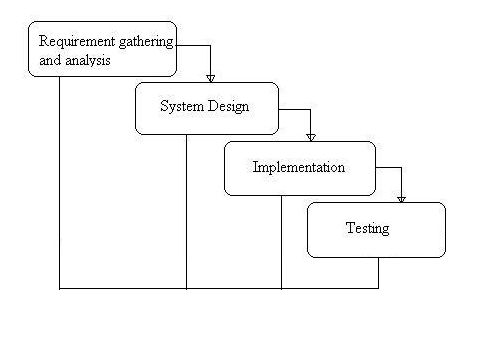
\includegraphics[width=1.0\textwidth, center]{images/waterfall_model.png}
		\foot{Waterfall-model (In our case it end on testing)}
\end{figure}


This model is easy to understand and use. It is mostly used with relatively small project where all requirements are well understood (returning to earlier stages of project from e.g testing might be very expansive so it is better not to move to another stage without debugging). Each stage is completed one at a time so they are not overlapping.

\newpage
\section{Technologies} \par
\Large\hspace{15pt}
Our application will written in C\# language. For app development we will use Visual 2013. As a graphic engine we will use WPF (Windows Presentation Foundation) which is based on .NET 3. It gives nice tools to divide project on GUI and logical parts what helps in creating clean code. This application is destined for Windows Vista and higher. 



\section{Used data structures}
\Large\hspace{15pt}
To store grid data we will use two nested lists of cells object(or just boolean).In C\# exploring elements in List is as fast as in simple table but it gives way more tools. List is easy to expand/shrink and has many search functions already implemented.
\newpage
\section{Description of algorithm}
\Large\hspace{15pt} 
\hspace{15pt}This product will be based on Conway's Game of Life automaton. It means that is hat two dimensions. It also has two states (ON and OFF). State of the cell will be decided by \textbf{rules}. Rules describe which cells in neighborhood (4,8 or 24 point) are important and how many of them have to be in "ON" state  to keep cell alive or dead. Overlapping rules are resolved by one of three logical operations (XOR,OR,AND).
We need two 2-dimensional matrices and one of which will start as "original" one. We will go through matrix with 2 loops where one will be placed in another. In each iteration of inner loop we will calculate cell state. Depending on neighborhood size, appropriate rule set will be chosen. We have to iterate through all rules in rule set and check which of them can be applied. 



If there is more than one of them, than we use predefined logic operation to resolve this conflict (conflict arises since we can also create rule for killing a cell).
in case where some of neighbors are outside the matrix, we virtually "stitch" left with right side and top with bottom border. For instance if neighborhood i exceeding top border, lacking neighbors are those adjacent to bottom border.


After calculating the state of a cell, it is saved to cell with the same index in second matrix. Calculation of a new generation ends up in setting second matrix as an original one and displaying it on the screen. 


\newpage
\section{Functionality}
\normalsize
	\begin{itemize}
	
	\item	
	Display visualization of cell movements - every step of components behavior must be
	shown on a grid.\\
	\item Change environment - by selecting them; there must be at least 3 types of
	environments: 4, 8, 24 points neighborhood. \\
	\item Introduce new rules - by adding new rules determining new behavior of cells. \\
	\item Change rules - by dynamically changing existing rules. \\
	\item Create new rules - by selecting neighborhood cells and how many of them should be
	alive in order to make the target cell either alive or dead.\\
	\item Select number of steps .\\
	\item Control simulation - by choosing options play, pause, stop or reset simulation. \\
	\item Observe movements step by step - by rewinding cells movement on click, depending on
	the selected number of steps. \\
	\item Resolve conflicts when there are contradicting rules - by selecting one of them or
	selecting one of the logical operations (XOR, OR, AND) to be performed on them, for
	example rule 1 OR rule 2. \\
	\item Change grid's size - by option to zoom in/zoom out the visualisation.\\
	\item Load known automaton - for example Langton's ant. \\	
	\item Display information - by showing for example time of simulation (in seconds), number
	of cells alive. \\			
	\end{itemize}
\newpage
\section{Class diagram / program structure}
\Large\hspace{15pt} 
This class diagram is a simple visualization  of classes in our program. Person implementing these classes is free to divide them to smaller ones.
\begin{figure}[h!]
		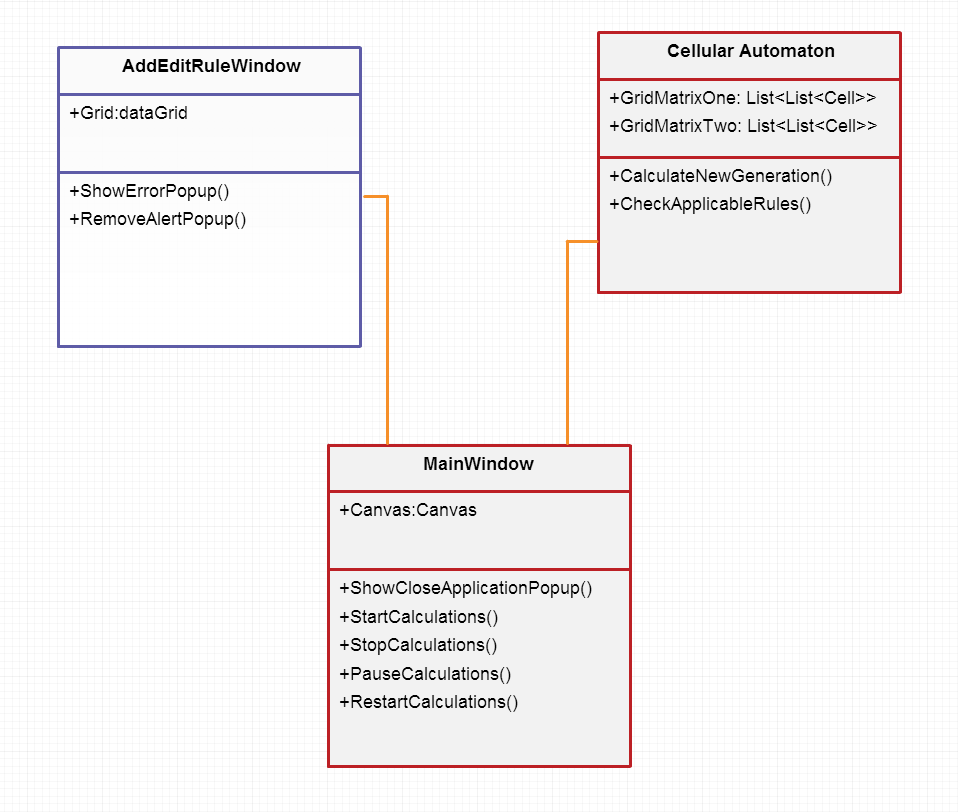
\includegraphics[width=1.5\textwidth, center]{images/Class_Diagram}
\end{figure}
\newpage
\section{Use cases}
Use case for user in main menu.
\begin{figure}[h!]
		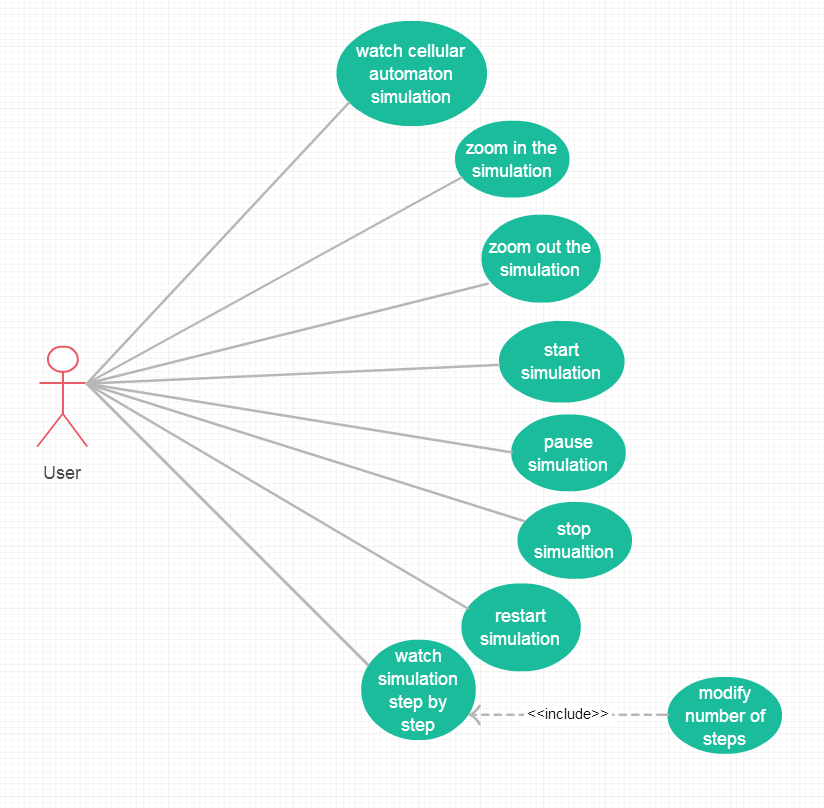
\includegraphics[width=1.3\textwidth, center]{images/user_usecase_diagram.png}
\end{figure}
\newpage
Use case for user in Add/Edit menu.
\begin{figure}[h!]
		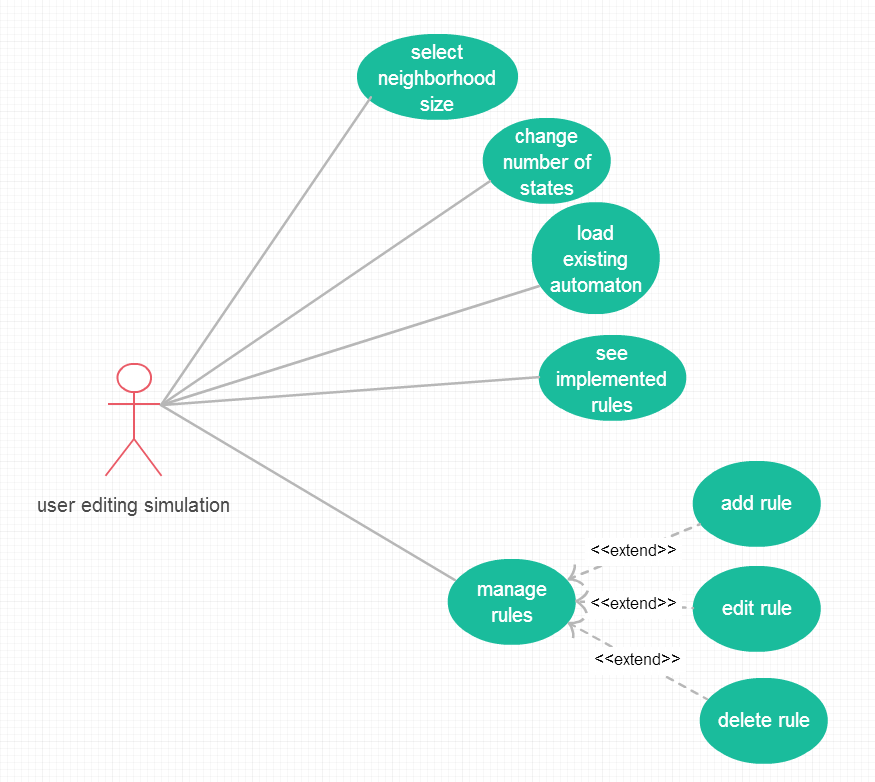
\includegraphics[width=1.3\textwidth, center]{images/user_editing_simulation_usecase_diagram.png}
\end{figure}


\newpage


\section{States diagram}
Simple state diagram describing behavior of program in general.
\begin{figure}[h!]
		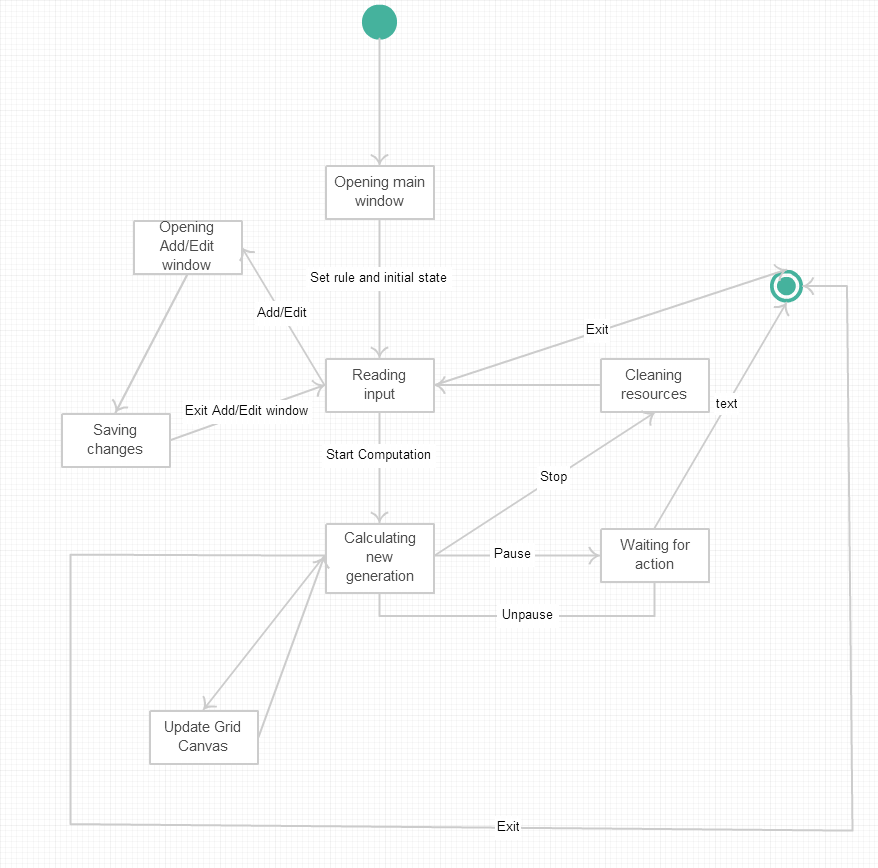
\includegraphics[width=1.3\textwidth, center]{images/state_diagram.png}
\end{figure}
\newpage

\section{Graphical user interface mock-up}
\begin{figure}[h!]
		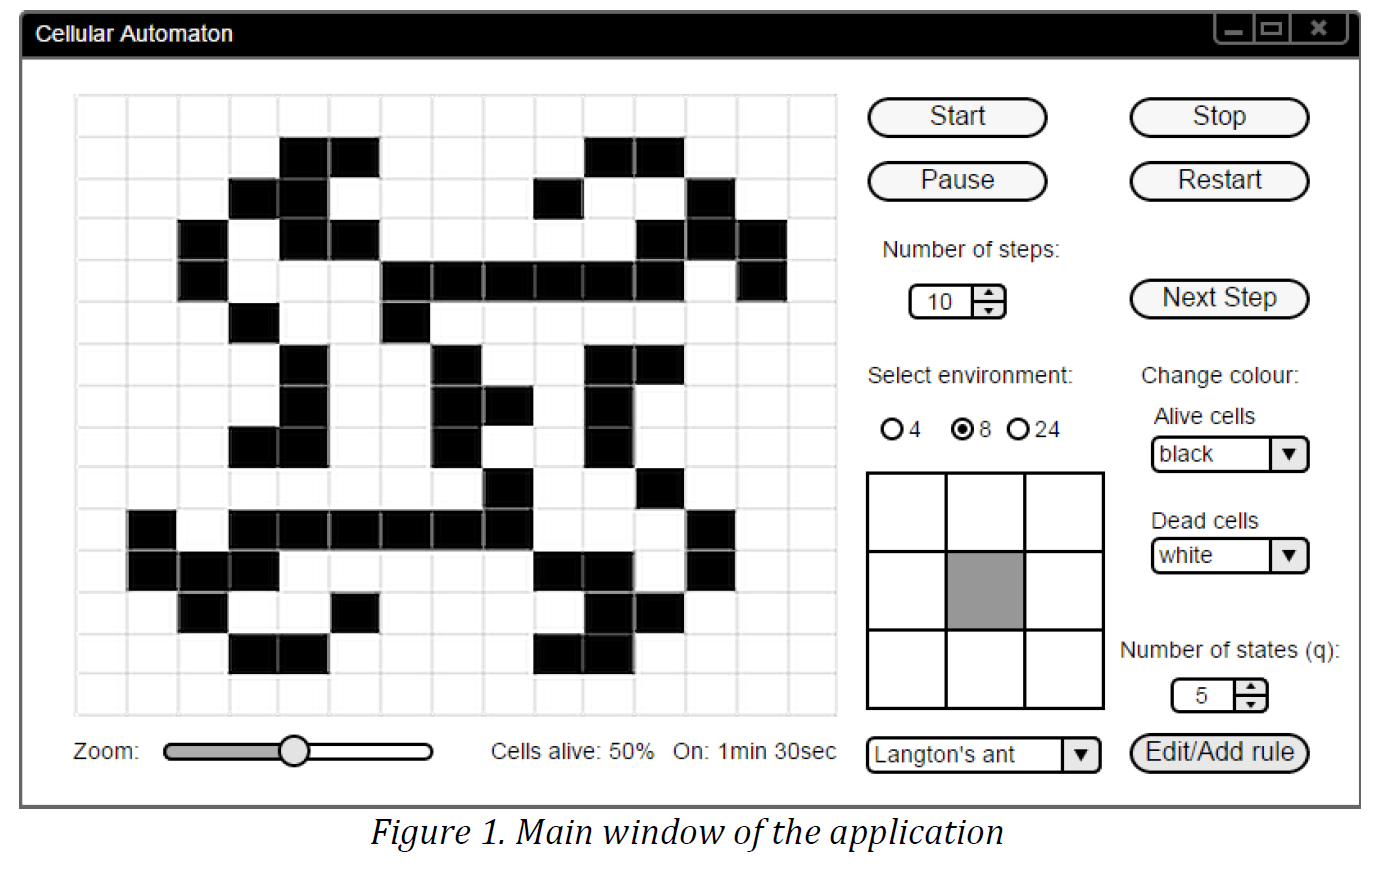
\includegraphics[width=1.0\textwidth, center]{images/Figure1.png}
\end{figure}
\begin{figure}[h!]
		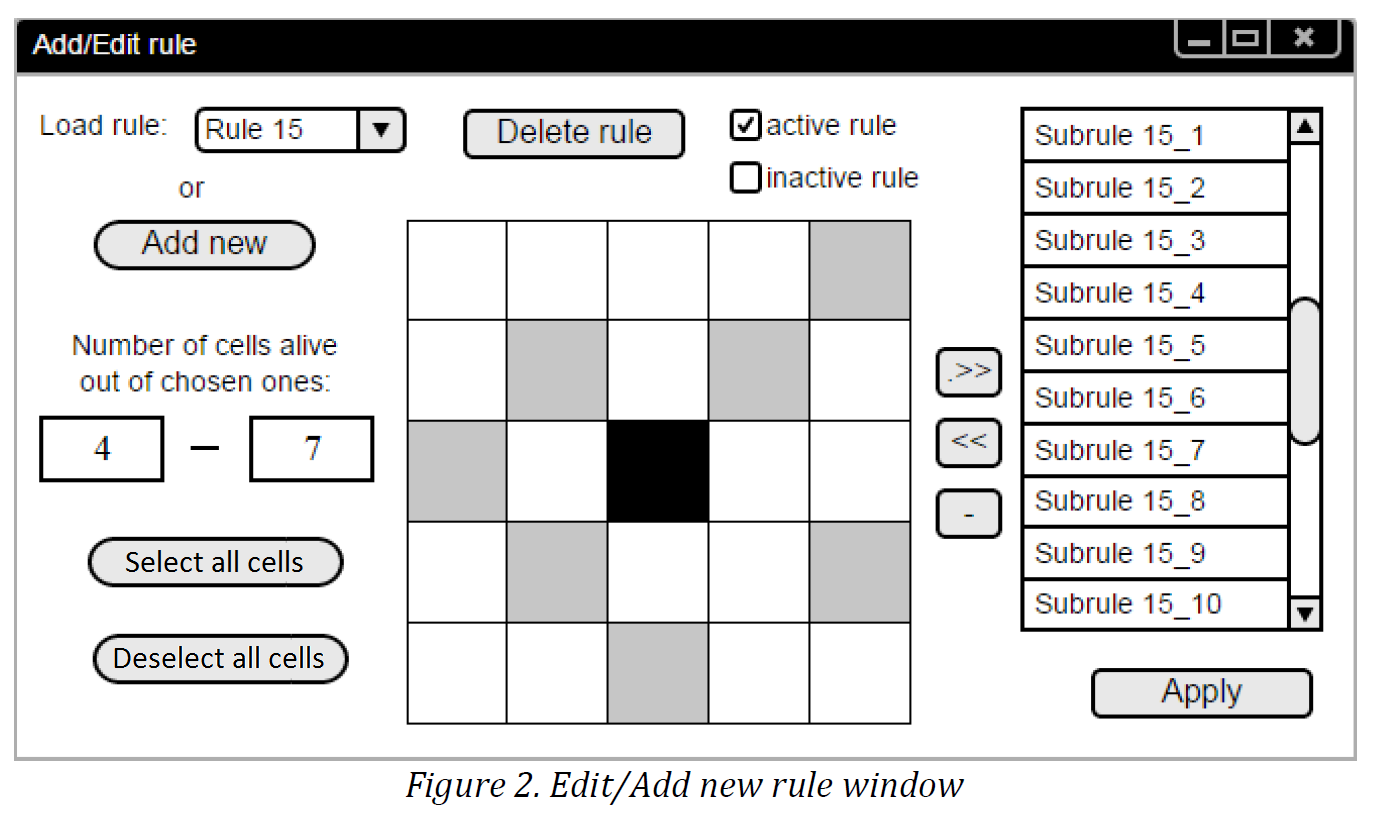
\includegraphics[width=1.0\textwidth, center]{images/Figure2.png}
\end{figure}
\begin{figure}[h!]
		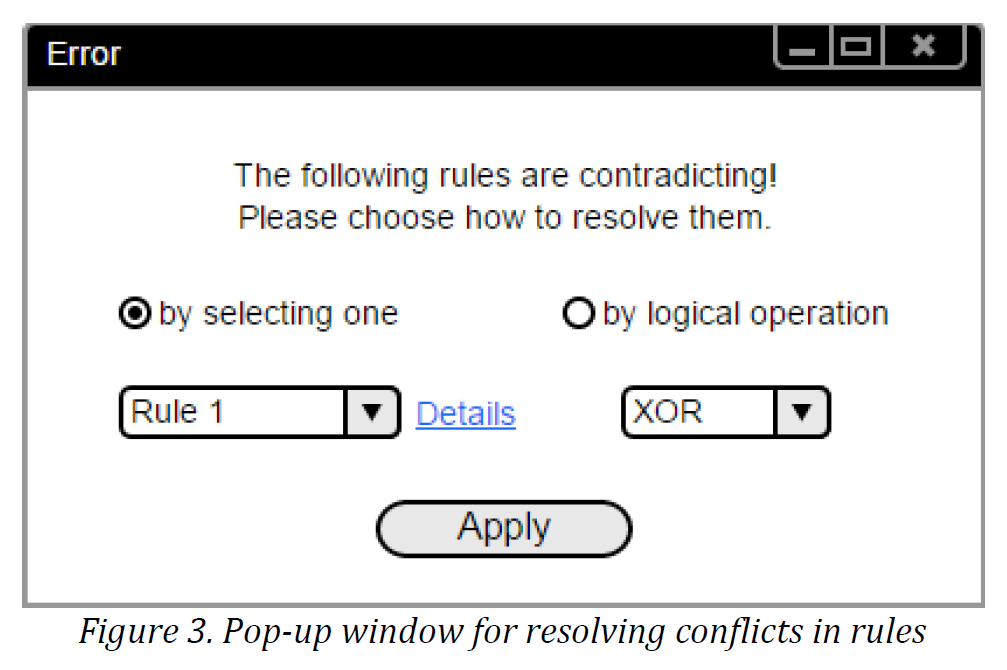
\includegraphics[width=0.8\textwidth, center]{images/Figure3.png}
\end{figure}
\begin{figure}[h!]
		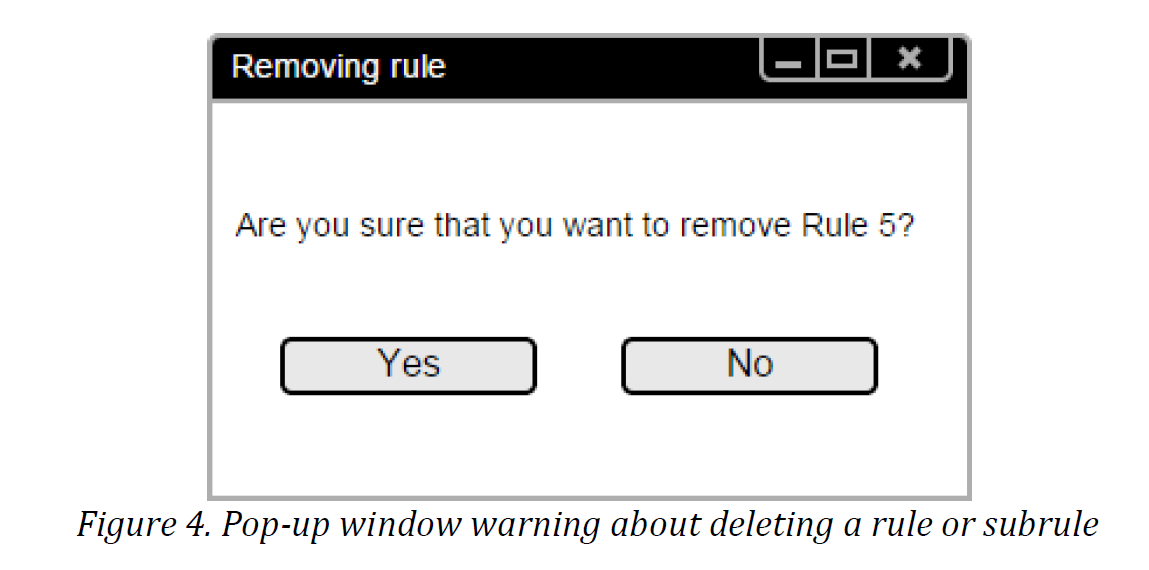
\includegraphics[width=1.0\textwidth, center]{images/Figure4.png}
\end{figure}

\begin{figure}[h!]
		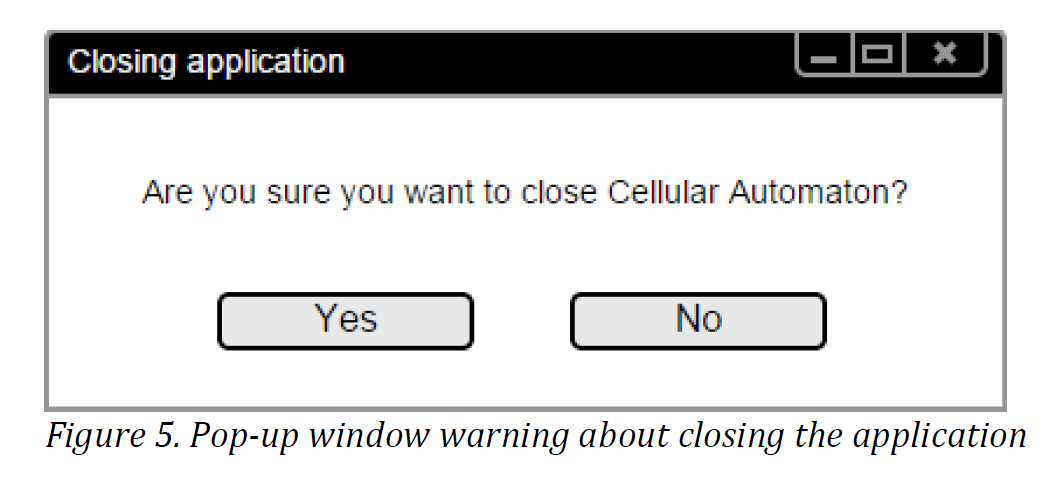
\includegraphics[width=0.8\textwidth, center]{images/Figure5.png}
\end{figure}

\newpage

\section {Summary}

This technical documentation has been made basing on Business analysis made by Mai Viet Ba. "Functionality" and "Graphical user interface mock-up" has been copied since these informations are very important from technical aspect.

Application created basing on this documentation should be very fast, user friendly and eye pleasing. The biggest drawback will be support for only one computer system (it also might be open through "Wine" on Linux but it's not an official solution so it might not work properly).


\end{document}
